\documentclass[12pt, a4paper]{article}
\usepackage{xltxtra}
\usepackage{polyglossia}
\setmainlanguage{russian}
%\setotherlanguage{english}


\setmainfont{Times New Roman}
\setromanfont{Times New Roman} 
\setsansfont{Arial} 
\setmonofont{Courier New} 

\newfontfamily{\cyrillicfont}{Times New Roman} 
\newfontfamily{\cyrillicfontrm}{Times New Roman}
\newfontfamily{\cyrillicfonttt}{Courier New}
\newfontfamily{\cyrillicfontsf}{Arial}


\usepackage{graphicx}
\usepackage{wordlike}
\usepackage{hyperref}
\title{Навигация и концепция административного блока}
\author{Ефим Маневич}
\date{25 июля 2022}

\begin{document}
\maketitle

\section{Навигация в приложении}

Навигация в приложении происходит с помощью древовидного меню, меню вызывается по кнопке слева на
главной панели приложения. 

\begin{center}
    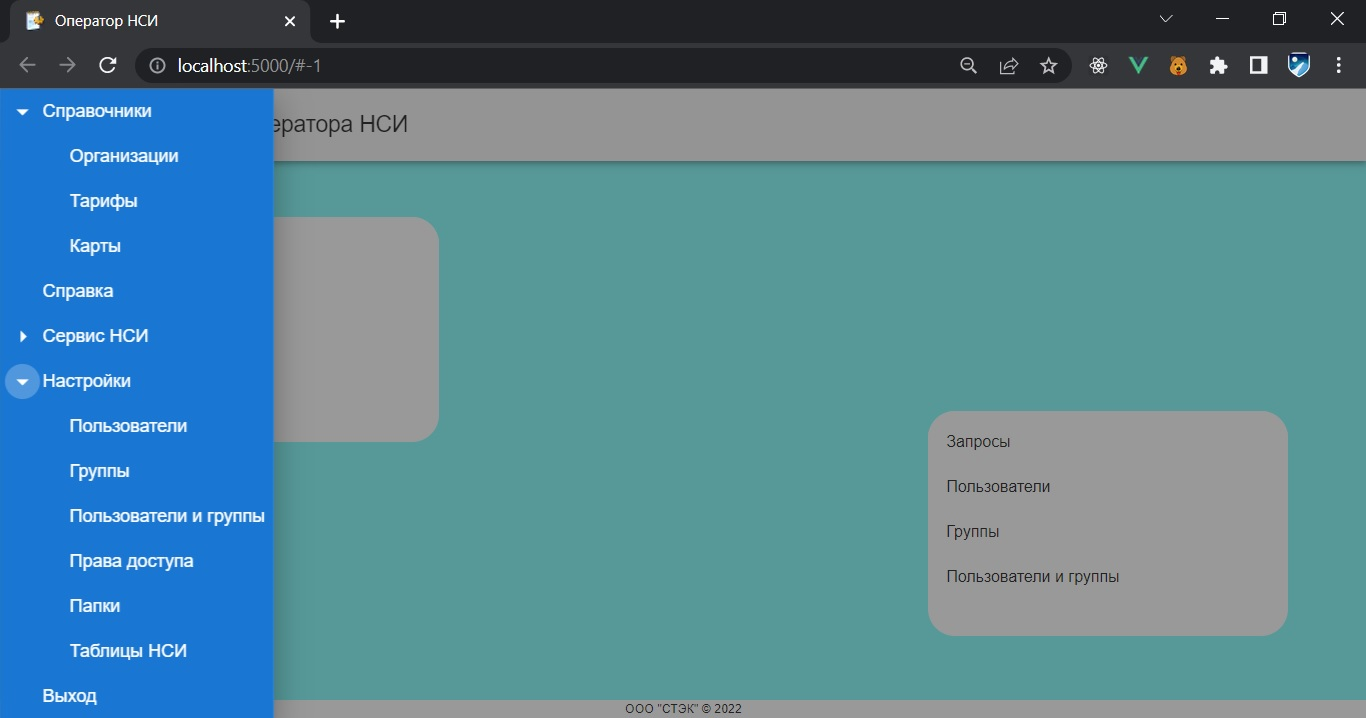
\includegraphics [width=\textwidth] {p1.png}
\end{center}

Меню приложения разделено на секции. 

Разделы "Настройка" и "СервисНСИ" доступны только администратору:

\begin{center}
    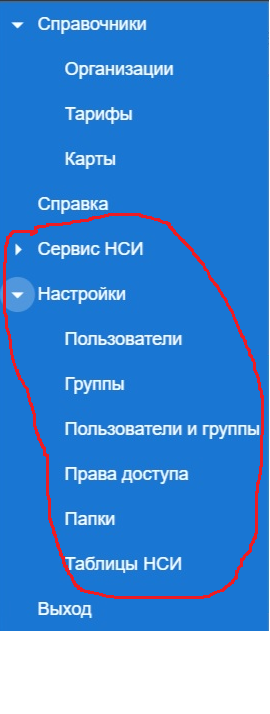
\includegraphics {p2.png}
\end{center}

Администратор может добавить произвольные любые другие секции и пункты меню. 
Эти пункты меню можно сделать доступными пользователям из группы "Операторы":

\begin{center}
    
\includegraphics  {p3.png}
\end{center}

Новые пункты меню, которые добавляет администратор, предназначены для вывода данных справочника в табличной форме.

Справочники для пользователей создаются на основе источников данных указанных в разделе "СервисНСИ". 

В разделе "СервисНСИ" три пункта меню:
\begin{itemize}
    \item [1] {Коннекторы}
    \item [2] {Запросы}
    \item [3] {Тест АПИ}
\end{itemize}

\section{Создание нового пункта меню}
Для того чтобы создать новый справочник доступный пользователю, необходимо выбрать источник данных из таблицы
"СервисНСИ/Запросы", в дальнейшем нас будет интересовать имя запроса:

\begin{center}
    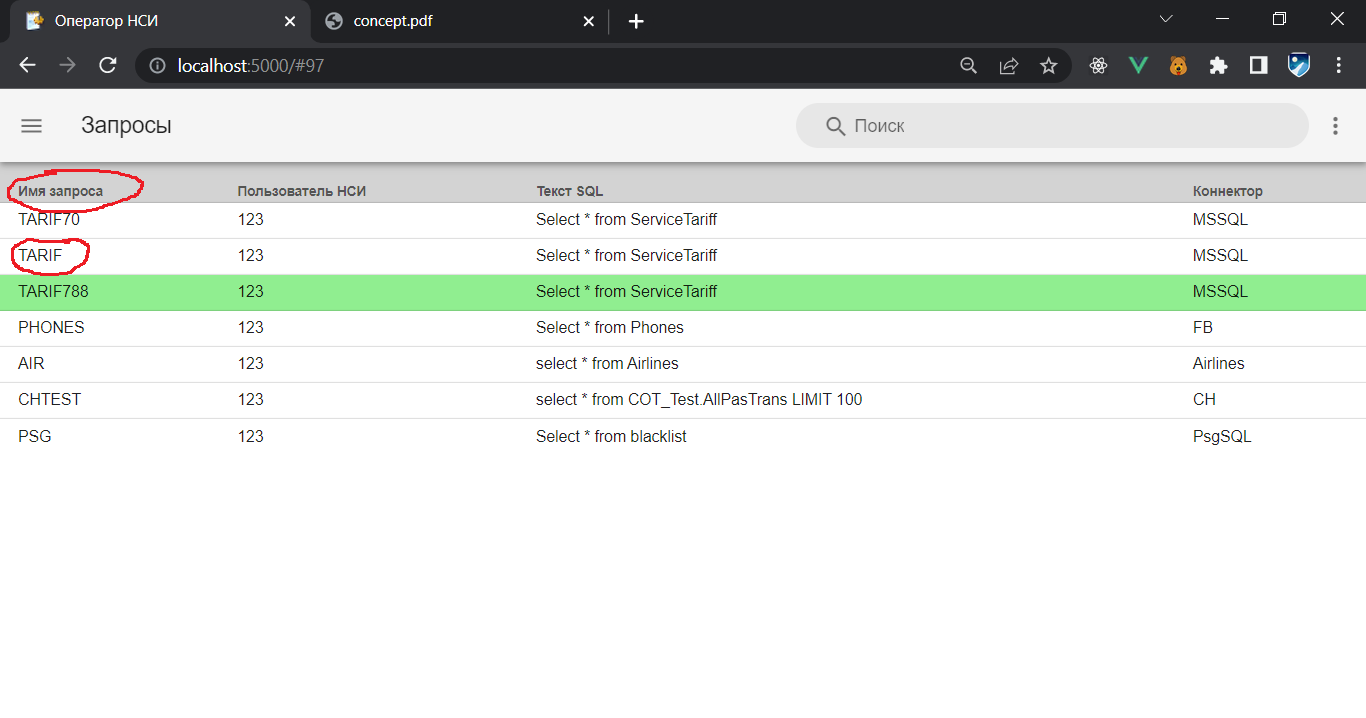
\includegraphics [width=\textwidth] {p4.png}
\end{center}

В общих чертах схема добавление пункта меню (справочника) доступного оператору такова:

\begin{itemize}
    \item [1] {В форме "Настройки/Таблицы" добавляем новую таблицу, причем имя таблицы должно совпадать с выбранным именем источника данных}
    \item [2] {В форме "Настройки/Папки" добавляем новый пункт меню в котором содержится ссылка на созданную таблицу}
    \item [3] {В форме права доступа раздаются права на новый пункт меню. Права раздаются пользователям или группам пользователей.}
\end{itemize}

\section{Пользователи, группы, права доступа}
Администратор создает новых пользователей, создает новые группы. В группу могут быть добавлены другие пользователи или
группы. Для ведения базы пользователей, групп предназначены пункты меню: Настройки/Пользователи", "Настройки/Группы",
"Настройки/Пользователи и группы" (для редактирования состава группы).

Права доступа принимают два значения 0/1. 0 - объект недоступен, 1 - доступен. 
Объектами доступа в данном приложении являются пункты основного меню.

Подробная инструкция администратора будет представлена отдельно.

\section{Главная страница приложения}
На главной странице выводится 8 первых доступных пользователю пунктов меню. Ссылки выводятся в двух блоках
по 4 записи.

\begin{center}
    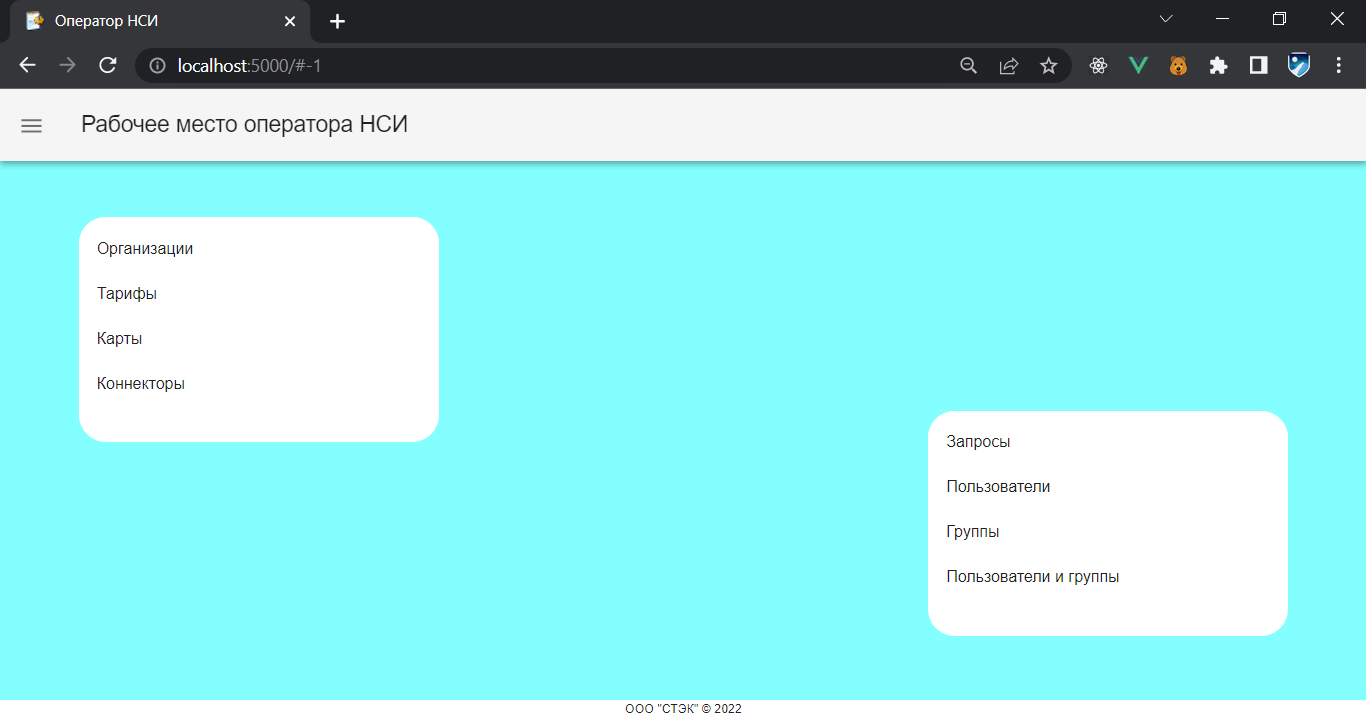
\includegraphics [width=\textwidth] {p5.png}
\end{center}

\section{Приложение}
В настоящий момент в приложении реализована изложенная логика. Можно тестировать приложение по адресу:

\url{http://51.250.44.37:5000/}

Вход для администратора:

Логин: Admin

Пароль: 123

Вход для оператора:

Логин: User

пароль: 123



\end{document}